\chapter{METODOLOGÍA Y MARCO TECNOLÓGICO}

El presente capítulo describe el enfoque metodológico y las decisiones tecnológicas adoptadas para el desarrollo de la plataforma Bebras Bolivia. En primer lugar, se analizan plataformas nacionales de referencia con el propósito de identificar patrones de arquitectura, módulos funcionales y criterios de diseño reutilizables. Posteriormente, se examina la naturaleza de los sistemas de gestión de concursos en línea, distinguiéndolos de otras plataformas educativas y precisando los requisitos operativos que condicionan su implementación.

Finalmente, se presentan las herramientas y tecnologías seleccionadas para la construcción del sistema, justificando su elección en función de criterios de rendimiento, mantenibilidad, coherencia de pila y adecuación al contexto del proyecto. Esta exposición metodológica y tecnológica permite fundamentar la solución propuesta no solo desde el punto de vista conceptual, sino también desde su viabilidad práctica e implementación efectiva.

\section{RETROINGENIERÍA DE PLATAFORMAS BEBRAS DE REFERENCIA}

Con el propósito de fundamentar las decisiones de diseño funcional, arquitectónico y de interfaz de la plataforma propuesta para Bebras Bolivia, se realizó un proceso de retroingeniería sobre un conjunto de implementaciones nacionales del Desafío Bebras. Este proceso no se limitó a una descripción general de los sitios o repositorios disponibles, sino que buscó identificar de manera sistemática los componentes, patrones de organización, módulos funcionales y estrategias de interacción más relevantes de cada plataforma analizada.

La selección de los casos de estudio respondió a criterios complementarios: disponibilidad de código fuente o información técnica pública, grado de madurez de la implementación, representatividad dentro del ecosistema Bebras y utilidad como referencia para el contexto boliviano. A partir de esta revisión, fue posible reconocer fortalezas particulares en cada plataforma y extraer de ellas los elementos más valiosos para la definición de la propuesta tecnológica del presente trabajo. En consecuencia, la retroingeniería realizada no tuvo como finalidad replicar una solución existente, sino sintetizar buenas prácticas dispersas en distintas implementaciones nacionales para integrarlas en un sistema propio, coherente con los requerimientos de Bebras Bolivia.

\subsection{Plataforma de Francia --- Castor Informatique}

La implementación francesa, \emph{Castor Informatique}, mantenida por France-IOI, constituye una de las referencias más consolidadas dentro del ecosistema Bebras y dispone de código fuente accesible públicamente \parencite{bebrasfrancia}. El análisis de su estructura permitió identificar una separación clara entre módulos de concurso, docentes y preguntas, así como una estrategia orientada a optimizar la entrega de contenido mediante generación o compilación previa de materiales de prueba.

Desde la perspectiva de retroingeniería, el principal aporte de esta plataforma radica en su eficiencia para servir contenido y en la organización clara de sus componentes funcionales. Para Bebras Bolivia, esta referencia resultó especialmente útil en la definición de estrategias de entrega de contenido y en la inspiración de un esquema modular para separar áreas públicas, administrativas y de evaluación.

\subsection{Plataforma de Bélgica --- Rasbeb2}

La plataforma belga \emph{Rasbeb2}, disponible bajo licencia MIT \parencite{bebrasbelgica}, presenta una arquitectura orientada a la gestión integral del concurso. Su implementación en Java y su organización por módulos administrativos, tareas interactivas y documentación permitieron identificar una estructura robusta para el manejo de procesos internos del sistema.

El principal valor extraído de esta plataforma fue su diseño modular aplicado al flujo del concurso, particularmente en la separación entre inscripción, administración, ejecución y evaluación. Aunque no se adoptó su base tecnológica, su organización interna aportó criterios relevantes para estructurar el CMS de Bebras Bolivia desde una lógica funcional más que desde una lógica de simple desarrollo web.

\subsection{Plataforma de Perú --- Bebras Perú}

La plataforma de Bebras Perú \parencite{bebrasperu} ofrece una referencia importante desde el punto de vista comunicacional e institucional. Su sitio prioriza la presentación pública de información para docentes, instituciones educativas y participantes, organizando con claridad niveles, recursos, orientaciones y mecanismos de inscripción.

A partir de la retroingeniería de esta plataforma, se identificó como fortaleza principal la claridad en la arquitectura de información orientada a usuarios no técnicos. Este aspecto fue considerado especialmente valioso para el diseño de la \emph{landing page} de Bebras Bolivia, ya que evidencia la necesidad de estructurar el contenido de manera diferenciada para coordinadores institucionales, docentes, estudiantes y familias.

\subsection{Plataforma de Estados Unidos --- Bebras Computing Challenge}

La plataforma de \textcite{bebraseeuu} combina un entorno de práctica abierta con acceso a tareas de ediciones anteriores y un espacio de gestión dirigido a coordinadores institucionales. Su interfaz organiza de forma clara las categorías, el formato del concurso y los mecanismos de participación, al mismo tiempo que ofrece una experiencia de resolución de ejercicios bien definida.

Desde la retroingeniería realizada, su principal aporte fue el modelo de interacción del módulo de ejercicios, especialmente en aspectos como la presentación del problema, la navegación entre tareas, la retroalimentación al usuario y la integración entre práctica y evaluación. Estos elementos sirvieron como referencia directa para definir la experiencia de uso esperada en el módulo de resolución de tareas de Bebras Bolivia.

\subsection{Síntesis de aportes extraídos de la retroingeniería}

La retroingeniería de las plataformas analizadas permitió concluir que no existe una única implementación que resuelva de manera integral todos los requerimientos identificados para Bebras Bolivia. Sin embargo, cada una de las referencias estudiadas aporta fortalezas concretas que pueden ser integradas en una propuesta propia. En este sentido, el presente proyecto no se plantea como una réplica de ninguna plataforma existente, sino como una síntesis de buenas prácticas funcionales, arquitectónicas y de interfaz observadas en distintas implementaciones nacionales del ecosistema Bebras.

\begin{table}[H]
\centering
\caption[Elementos recuperados de plataformas Bebras de referencia]{Elementos recuperados mediante retroingeniería de plataformas Bebras de referencia y su aplicación en Bebras Bolivia}
\label{tab:retro_bebras}
\renewcommand{\arraystretch}{1.25}
\begin{tabular}{|p{3.5cm}|p{4.8cm}|p{6cm}|}
\hline
\textbf{Plataforma} & \textbf{Elemento rescatado} & \textbf{Aplicación} \\ \hline
Castor Informatique & Separación entre concurso, docentes y banco de preguntas; publicación eficiente de contenidos & Base para dividir el sistema en módulos administrativos, académicos y de evaluación, y para orientar la entrega optimizada de tareas y recursos \\ \hline
Rasbeb2 & Organización modular del flujo del concurso y soporte para tareas interactivas & Referencia para estructurar los procesos de inscripción, ejecución, corrección y administración del concurso dentro del CMS \\ \hline
Bebras Perú & Arquitectura de información clara para docentes, instituciones y postulantes & Base para diseñar la \emph{landing page} y ordenar la comunicación institucional según tipo de usuario \\ \hline
Bebras Computing Challenge & Presentación de tareas, práctica previa y navegación entre ejercicios & Referencia para definir la experiencia del participante en el módulo de resolución de tareas y práctica \\ \hline
\end{tabular}
\end{table}

\section{SISTEMAS DE GESTIÓN DE CONCURSOS EN LÍNEA}

Un sistema de gestión de concursos en línea es una plataforma web que administra de manera integral el ciclo de vida de una competencia: el registro de participantes e instituciones, la configuración y distribución de pruebas, la ejecución controlada de exámenes en sesiones con tiempo limitado, la evaluación automática de respuestas y la publicación de resultados. Este tipo de sistemas se articula en torno a tres funciones esenciales: la autenticación segura de los participantes, la gestión del banco de preguntas y el motor de evaluación automática. Estos tres componentes están presentes en todas las implementaciones nacionales de Bebras analizadas y definen igualmente los módulos centrales del sistema desarrollado en este proyecto.

A diferencia de un sistema de gestión de aprendizaje (\textit{Learning Management System}, LMS) de propósito general, un sistema de gestión de concursos educativos debe garantizar condiciones equivalentes para todos los participantes durante la ejecución de la prueba: disponibilidad simultánea para múltiples sesiones concurrentes, control estricto del tiempo por participante y registro confiable de respuestas ante posibles interrupciones de conectividad. Estos requisitos condicionan directamente las decisiones de arquitectura del sistema propuesto.

La distinción funcional entre un sistema de gestión de concursos y un LMS se ilustra en la Figura~\ref{fig:cms_vs_lms}.

\begin{figure}[htbp]
    \centering
    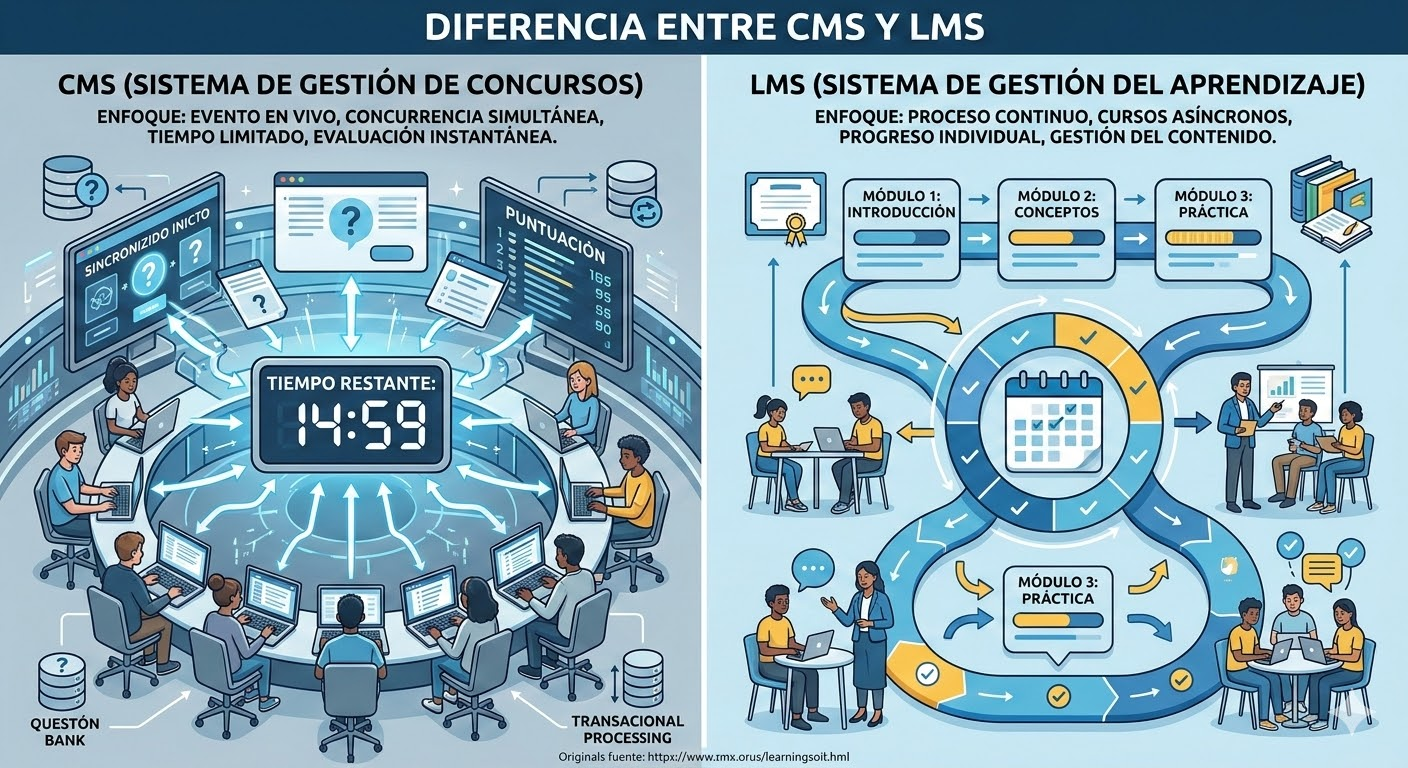
\includegraphics[width=0.70\textwidth]{assets/cms_vs_lms.jpg}
    \caption[Comparación entre CMS y LMS]{Comparación conceptual entre un \textit{Contest Management System} y un \textit{Learning Management System} - Elaboración propia}
    \label{fig:cms_vs_lms}
\end{figure}

\section{METODOLOGÍA DE ANÁLISIS Y DISEÑO}

La metodología adoptada en este trabajo combina revisión documental, análisis comparativo de plataformas de referencia y definición de una arquitectura ajustada a los requisitos funcionales y no funcionales del proyecto. En una primera etapa, se realizó una revisión de literatura especializada sobre pensamiento computacional, el modelo Bebras y la construcción de tareas educativas de informática. En una segunda etapa, se analizaron distintas plataformas nacionales de Bebras con el fin de identificar módulos recurrentes, patrones de interacción y decisiones arquitectónicas relevantes.

Sobre la base de este análisis, se procedió a definir los módulos que conforman la propuesta tecnológica para Bebras Bolivia: una \emph{landing page} orientada a la comunicación institucional, un sistema de inscripción para instituciones y participantes, un módulo de administración de exámenes, un entorno de resolución de tareas y un módulo de construcción y gestión de ejercicios. Finalmente, se seleccionó una pila tecnológica coherente con los requerimientos de rendimiento, mantenibilidad y escalabilidad identificados durante el proceso.

\section{MARCO TECNOLÓGICO}

El objetivo técnico central de este proyecto es el desarrollo de un sistema capaz de administrar de extremo a extremo el ciclo de vida del Desafío Bebras Bolivia: inscripción de instituciones y participantes, configuración y distribución de exámenes, ejecución controlada de pruebas en línea, registro automático de respuestas y consulta de resultados. A este sistema se suma un módulo de \textit{landing page} con capacidades propias de gestión de contenido, orientado a la comunicación institucional del desafío. La selección de tecnologías responde a criterios de rendimiento, coherencia de pila y mantenibilidad a largo plazo, considerando que ambos módulos deben operar de manera integrada sobre el mismo entorno de ejecución.

\subsection{Astro}

Astro fue seleccionado para el módulo de \textit{landing page} por su enfoque en rendimiento y generación de contenido estático. \textcite{astro} destaca su modelo \textit{server-first} y la \emph{Islands Architecture}, que hidrata solo los componentes interactivos y reduce JavaScript en cliente. Además, su integración con \textit{Content Collections} permite administrar contenido institucional de forma tipada y mantenible, en coherencia con la pila basada en Bun.

\subsection{Bun}

Bun se utiliza como entorno de ejecución unificado para JavaScript y TypeScript en el proyecto. \textcite{bun} lo describe como una alternativa de alto rendimiento que integra \textit{runtime}, gestor de paquetes y herramientas de desarrollo en una sola tecnología. Esta unificación simplifica la operación del sistema y reduce tiempos de ejecución y despliegue frente a cadenas de herramientas separadas.

\subsection{Express}

Express se eligió para la capa API del sistema por su arquitectura modular basada en \textit{middleware}. \textcite{express} resalta su flexibilidad para estructurar rutas, validaciones y control de errores sin imponer una arquitectura rígida. Esto ofrece una base adecuada para implementar flujos como autenticación, gestión de sesiones de examen y registro de respuestas dentro de una plataforma de este tipo.

\subsection{Prisma ORM}

Prisma ORM se adoptó para el acceso a datos por su tipado estático en TypeScript y su manejo controlado de migraciones. \textcite{prisma} identifica como componentes centrales Prisma Client, Prisma Migrate y Prisma Studio. En este proyecto, \texttt{schema.prisma} funciona como fuente única de verdad del modelo, lo que mejora la consistencia del esquema y reduce errores de consulta en la integración con MariaDB.

\subsection{MariaDB}

MariaDB fue seleccionado como motor relacional del sistema por su madurez, licencia libre y compatibilidad con MySQL. De acuerdo con \textcite{mariadb}, mantiene compatibilidad de interfaces y bibliotecas, incorporando mejoras para entornos productivos. Su compatibilidad con Prisma ORM, mediante el conector de MySQL, lo convierte en una base sólida para la persistencia de datos del sistema.

La selección de las tecnologías descritas no respondió únicamente a criterios funcionales aislados, sino a una evaluación conjunta de sostenibilidad técnica, consumo de recursos, capacidad de escalamiento y afinidad con la experiencia previa del equipo de desarrollo. En este sentido, se priorizaron herramientas consolidadas, activamente mantenidas y adecuadas para una infraestructura moderada, evitando depender de soluciones excesivamente recientes o inciertas en su continuidad. La Tabla~\ref{tab:criterios_tecnologias} sintetiza estos criterios de selección.

\begin{table}[H]
\centering
\caption[Criterios de selección de tecnologías]{Criterios que fundamentan la selección de las tecnologías del proyecto}
\label{tab:criterios_tecnologias}
\renewcommand{\arraystretch}{1.2}
\begin{tabular}{|p{2.8cm}|p{4.2cm}|p{6.5cm}|}
\hline
\textbf{Tecnología} & \textbf{Criterio principal} & \textbf{Justificación} \\ \hline
Astro & Eficiencia y optimización en frontend & Adecuado para una \emph{landing page} con contenido mayormente estático, reduciendo carga innecesaria en cliente y servidor. \\ \hline
Bun & Rendimiento y proyección técnica & Permite un entorno unificado con buen desempeño y menor sobrecarga operativa, manteniendo una tecnología activa y con proyección de continuidad. \\ \hline
Express & Estabilidad y dominio del equipo & Proporciona una base ligera, madura y conocida por el equipo, lo que facilita el desarrollo, mantenimiento y crecimiento del backend. \\ \hline
Prisma ORM & Mantenibilidad del modelo de datos & Su tipado y control de migraciones favorecen la consistencia del sistema y reducen errores durante el desarrollo y la evolución del proyecto. \\ \hline
MariaDB & Madurez y bajo costo operativo & Es una solución relacional estable, eficiente en recursos y adecuada para operar sobre infraestructura moderada sin sacrificar confiabilidad. \\ \hline
\end{tabular}
\end{table}